\documentclass[10pt,]{article}
\usepackage{lmodern}
\usepackage{amssymb,amsmath}
\usepackage{ifxetex,ifluatex}
\usepackage{fixltx2e} % provides \textsubscript
\ifnum 0\ifxetex 1\fi\ifluatex 1\fi=0 % if pdftex
  \usepackage[T1]{fontenc}
  \usepackage[utf8]{inputenc}
\else % if luatex or xelatex
  \ifxetex
    \usepackage{mathspec}
  \else
    \usepackage{fontspec}
  \fi
  \defaultfontfeatures{Ligatures=TeX,Scale=MatchLowercase}
\fi
% use upquote if available, for straight quotes in verbatim environments
\IfFileExists{upquote.sty}{\usepackage{upquote}}{}
% use microtype if available
\IfFileExists{microtype.sty}{%
\usepackage{microtype}
\UseMicrotypeSet[protrusion]{basicmath} % disable protrusion for tt fonts
}{}
\usepackage[margin=1.0in]{geometry}
\usepackage{hyperref}
\hypersetup{unicode=true,
            pdftitle={Suggestions for improving invited speaker diversity to reflect trainee diversity},
            pdfborder={0 0 0},
            breaklinks=true}
\urlstyle{same}  % don't use monospace font for urls
\usepackage{graphicx,grffile}
\makeatletter
\def\maxwidth{\ifdim\Gin@nat@width>\linewidth\linewidth\else\Gin@nat@width\fi}
\def\maxheight{\ifdim\Gin@nat@height>\textheight\textheight\else\Gin@nat@height\fi}
\makeatother
% Scale images if necessary, so that they will not overflow the page
% margins by default, and it is still possible to overwrite the defaults
% using explicit options in \includegraphics[width, height, ...]{}
\setkeys{Gin}{width=\maxwidth,height=\maxheight,keepaspectratio}
\IfFileExists{parskip.sty}{%
\usepackage{parskip}
}{% else
\setlength{\parindent}{0pt}
\setlength{\parskip}{6pt plus 2pt minus 1pt}
}
\setlength{\emergencystretch}{3em}  % prevent overfull lines
\providecommand{\tightlist}{%
  \setlength{\itemsep}{0pt}\setlength{\parskip}{0pt}}
\setcounter{secnumdepth}{0}
% Redefines (sub)paragraphs to behave more like sections
\ifx\paragraph\undefined\else
\let\oldparagraph\paragraph
\renewcommand{\paragraph}[1]{\oldparagraph{#1}\mbox{}}
\fi
\ifx\subparagraph\undefined\else
\let\oldsubparagraph\subparagraph
\renewcommand{\subparagraph}[1]{\oldsubparagraph{#1}\mbox{}}
\fi

%%% Use protect on footnotes to avoid problems with footnotes in titles
\let\rmarkdownfootnote\footnote%
\def\footnote{\protect\rmarkdownfootnote}

%%% Change title format to be more compact
\usepackage{titling}

% Create subtitle command for use in maketitle
\newcommand{\subtitle}[1]{
  \posttitle{
    \begin{center}\large#1\end{center}
    }
}

\setlength{\droptitle}{-2em}

  \title{\textbf{Suggestions for improving invited speaker diversity to reflect
trainee diversity}}
    \pretitle{\vspace{\droptitle}\centering\huge}
  \posttitle{\par}
    \author{}
    \preauthor{}\postauthor{}
    \date{}
    \predate{}\postdate{}
  
\usepackage{booktabs}
\usepackage{longtable}
\usepackage{array}
\usepackage{multirow}
\usepackage[table]{xcolor}
\usepackage{wrapfig}
\usepackage{float}
\usepackage{colortbl}
\usepackage{pdflscape}
\usepackage{tabu}
\usepackage{threeparttable}
\usepackage{threeparttablex}
\usepackage[normalem]{ulem}
\usepackage{makecell}
\usepackage{caption}

\usepackage{helvet} % Helvetica font
\renewcommand*\familydefault{\sfdefault} % Use the sans serif version of the font
\usepackage[T1]{fontenc}

\usepackage[none]{hyphenat}

\usepackage{setspace}
\doublespacing
\setlength{\parskip}{1em}

\usepackage{lineno}

\usepackage{pdfpages}
\floatplacement{figure}{H} % Keep the figure up top of the page

\begin{document}
\maketitle

\vspace{30mm}

Running title: Suggestions for improving invited speaker diversity

\vspace{35mm}

Ada K. Hagan, Ph.D.\(^{1,2\dagger}\), Rebecca M. Pollet, Ph.D.\({^2}\),
and Josie Libertucci, Ph.D.\({^3}\)

\vspace{35mm}

\(\dagger\) To whom correspondence should be addressed:
\href{mailto:akhagan@alliancescc.com}{\nolinkurl{akhagan@alliancescc.com}}

1. Alliance SciComm \& Consulting, Linden, Michigan

2. Department of Microbiology \& Immunology, University of Michigan, Ann
Arbor, Michigan

3. Farncombe Family Digestive Health Research Institute, Department of
Medicine, McMaster University, Hamilton, Ontario, Canada

Figures: 1

Tables: 1

Financial support: Department of Microbiology \& Immunology, University
of Michigan

\newpage

\subsection{Conflict of Interest Notification
Page}\label{conflict-of-interest-notification-page}

\vspace{40mm}

All authors affirm that there are no conflicts of interest.

\newpage

\linenumbers

\subsection{Abstract}\label{abstract}

Within the field of biomedical research in the United States, the
proportion of underrepresented minorities at the full professor level
has remained consistently low, even though trainee demographics are
becoming more diverse. Underrepresented groups face a complex set of
barriers to achieving faculty status including imposter syndrome,
increased performance expectations, and patterns of exclusion.
Institutionalized racism and sexism have contributed to these barriers
and perpetuated policy that excludes underrepresented minorities. These
barriers can contribute to decreased feelings of belonging, which may
result in decreased retention of underrepresented minorities. Though
some universities have altered their hiring practices to increase the
number of underrepresented minorities in the applicant pool, these
changes have not been sufficient. Here we argue that departmental
invited seminar series can be used to provide trainees with scientific
role-models and increase their sense of belonging, while institutions
work towards more inclusive policy. In this study, we investigated the
demographics (gender and race) of invited seminar speakers over 5 years
to the Department of Microbiology and Immunology at the University of
Michigan. We also investigated current trainee demographics and compared
them to invited speaker demographics to gauge if our trainees are being
provided with representation of themselves. We found that invited
speaker demographics were skewed towards Caucasian men, and our trainee
demographics were not being represented. From these findings, we
proposed policy change within the department to address how speakers are
being invited with the goal of increasing speaker diversity to better
reflect trainee diversity. To facilitate this process, we developed a
set of suggestions and a web-based resource that allows scientists,
committees, and moderators to identify members of under-served groups.
These resources can be easily adapted by other fields or sub-fields to
promote inclusion and diversity at seminar series', conferences, and
colloquia.

\subsection{Keywords}\label{keywords}

inclusion, diversity, invited speakers, academia, graduate programs

\newpage

\subsection{Background}\label{background}

Long-standing systemic bias, sexism, and racism have contributed to the
under-representation of many racial and ethnic groups, as well as women,
in science, technology, engineering, and math (STEM) fields (1--4).
Specifically, within the field of biomedical research in the United
States, the proportion of underrepresented minorities at the full
professor level has remained consistently low at 4\% (survey data taken
from the NIH from 2001 to 2013) (5, 6). Similar discrepancies exist for
women in biomedical sciences as full professorships are currently held
mostly by men (7, 8). As demographics of faculty within the biomedical
sciences remains skewed towards Caucasian men, the demographics of
trainees (graduate students and postdocs) are becoming more diverse (5).

Policy changes are needed to support inclusion of all individuals,
particularly in the biomedical sciences, since underrepresented groups
face a complex set of barriers to achieving faculty status (9). For
example, the dedication of women, who have children, to their work is
perceived to be less than that of their colleagues, including men who
also have children (10--12). Historically under-represented minorities
in the United States (HURM), Asian/Asian-Americans, and women are all
held to stricter competency standards and report having to work harder
than Caucasian men to be perceived as legitimate scholars (13, 14).
Asian/Asian-Americans suffer from imposter syndrome at greater rates
than other marginalized groups and Asian women report a lack of sponsors
(15, 16). Increased performance expectations and patterns of exclusions
are consistent themes in studies characterizing the HURM faculty
experience (17, 18). While HURM and other marginalized groups share some
experiences, differences including varying rates of hiring and tenure
promotion mean that unique considerations are important for inclusion of
each group (3).

Here, we argue that in order to increase the retention of faculty from
marginalized groups at the professor level, universities should provide
trainees with visual representation of themselves as successful
scientists. Recent studies show that women in STEM benefit from women
role models through improved belonging and self-efficacy (19, 20).
Predictably, a lack of active inclusion decreases self-efficacy,
eventually resulting in decreased feelings of belonging for URMs (21).
However, as the demographics of trainees have become more diverse,
students who are not Caucasian men, are lacking role models.
Institutionalized racism and sexism (22), defined as policies, societal
norms, and ideologies that reinforce inequities, have played a large
role in access to, inclusion in, and hiring policies at U.S.
universities (23, 24). Accordingly, faculty from marginalized groups are
eliminated from the applicant pool and subsequent hires, leaving
university policies and practices to be predominantly created by
Caucasian men. Thus, institutionalized racism and sexism are perpetuated
(25, 26). Universities have begun adjusting hiring practices and
creating initiatives to address inequitable hiring practices, but have
had limited results (27). Considering that most faculties within the
U.S. are still skewed towards Caucaisan men, invited seminar series are
a possible tool to provide marginalized trainees with representation of
themselves as successful scientists.

Invited seminar series are common within biomedical departments across
the United States (28). Usually, seminar series' consist of faculty
members selecting a scientist from another institution to visit their
university and present their research, as well as meet with other
faculty members and trainees. Named lectureships follow the same format
but are decided by committee and are considered more prestigious because
they are named in honor of prominent local scientists. These seminar
series and lectureships provide an opportunity for trainees to be
exposed to research outside of their department. Additionally, being an
invited speaker provides the scientist with an opportunity to make
future collaborations and build their own curriculum vitae (CV).
Scientists invited to give seminars are widely regarded as successful
and the top in their field, providing an opportunity for trainees to be
exposed to successful scientists in that field. Some studies have
examined the addition of more women speakers at conferences to promote
inclusion (29--31), however, we have only identified one other study
that has focused on invited speakers at universities (28). In their
study, Nittrouer et al, examined 3,652 talks at 50 U.S. institutions in
2013 - 2014 and found that women faculty are less likely to be invited
speakers (28). We have not been able to identify any publications
examining scientific speaker diversity beyond gender or how department
speaker series compares to trainee diversity in that department.

In this study, we examine and compare the demographics of invited
speakers to Caucasian men in the Department of Microbiology and
Immunology at the University of Michigan. Additionally, we compare
invited-speaker demographics to the current trainee demographics to
gauge if trainee demographics are being represented throughout the
seminar series. Following our investigation, we proposed a policy change
to the Department of Microbiology and Immunology in how invited speakers
are selected to promote inclusion in our department and reduce
unconscious bias. In order to facilitate inviting a more diverse group
of scientists, we developed a set of resources that allow scientists,
within the fields of microbiology and immunology, to self-identify as
having an under-represented or under-served identity including: HURM,
non-Caucasian/non-HURM (NCNH), or a Caucasian woman. These resources
will promote inclusion and diversity by providing greater representation
of all scientists and will provide hosts an opportunity to invite a more
diverse group of scientists.

\subsection{Methods}\label{methods}

Each academic year, each faculty member in the Department of
Microbiology and Immunology at the University of Michigan has the
opportunity to invite one speaker per year for a weekly seminar series.
Some of these seminar slots are dedicated to named lectureships, which
are decided by committee, and three trainee-invited speakers. We
analyzed the demographics of invited speakers and faculty hosts for five
academic years (Fall 2014 - Spring 2019), and compared them to the
current trainees when the data were analyzed (Spring 2019). Each speaker
was only counted once and those listed as departmental faculty members
or as a ``host'' at any point could not also be considered ``invited
speakers''. The list of faculty hosts was used as a proxy for faculty
demographics since as hosts, these faculty members are visible
representatives of the department. There were a total of \{\texttt{r}\}
invited speakers and paired hosts. The trainees were identified using
departmental email lists that included masters students, doctoral
students, and post-doctoral fellows. There were \{\texttt{r}\} students
and \{\texttt{r}\} post-doctoral fellows.

This is a retrospective study, thus speakers were not asked for their
identities at the time of visit. Instead we hand-coded proxy
demographics of the speakers, faculty hosts and trainees using first
names, publicly available photos, and CVs (32--36). Information from
CVs, such as undergraduate institutions (e.g., Puerto Rico vs mainland
U.S.) and activity in HURM groups (e.g., SACNAS) helped inform our
demographics by indicating identities that might be held by that
individual. Because these data were collected from publicly available
sources, this study was not submitted to an IRB for consideration. The
presenting gender of each individual was inferred using a binary system
(man/woman). Due to the low number of individuals in the study,
race/ethnicity demographics were only split into three groups:
Caucasian, Historically Under-represented Minority (HURM), and
Non-Caucasian/Non-HURM (NCNH), each with a binary (yes/no) possibility.
Caucasian was inferred using the current U.S. Census definition where
those of Middle Eastern, European, and Russian descent are included. URM
individuals include those of African-American, Indigenous American,
Alaskan/Hawaiian Native, Latinx and/or Hispanic heritage (20 U.S. Code
§\,1067k), we use the HURM designation to recognize the history of
enslavement and active oppression in the U.S.. The NCNH group
predominantly included Asian/Asian-Americans, but also African
immigrants (37).

Data were compiled and figures generated in R Statistical Software,
using relevant packages (38--50).

\subsection{Results}\label{results}

To understand the representation of women, we compared the proportion of
women in each academic role. At the trainee level, more than half of
students and postdoctoral fellows were women. That dropped to 46.77\% of
faculty hosts and 38.73\% of the invited speakers (Fig. 1A). Of 27
lectureships over the five year period, 37.04\% were awarded to women.

Our analysis identified an over-representation of Caucasian individuals
as hosting faculty and invited speakers (80\% each), relative to the
proportion of Caucasian trainees, which was 55\% (Fig. 1B). We also
observed declines in the representation of HURM and NCNH faculty and
speakers relative to the trainees (Fig 1B). HURM trainees made up 11\%
of the department, on track with the 11\% of U.S. microbiology and
immunology doctorates awarded in 2017 (51). However, only 8.5\% of
invited speakers, and none of the hosting faculty, were HURM scientists.
NCNH trainees were 34\% of department students and postdocs (versus 22\%
of U.S. microbiology and immunology doctorates in 2017), but only 19\%
of hosting faculty and 10.5\% of invited speakers (51).

The more prestigious invited speaker lectureships were also dominated by
Caucasian scientists, who comprised 81.48\% of those awarded (Fig. 1C).
HURM and NCNH scientists were awarded 3 and 2 lectureships,
respectively. Because the intersection of identities can compound biases
and outcomes, we further examined the lectureships by gender and
race/ethnicity status (52). Caucasian men and women accounted for
44.44\% and 37.04\% of the lectureships, respectively. Just 18.52\% of
lectureships were held by non-Caucasian men while none were held by
non-Caucasian women (Fig. 1D).

\subsection{Discussion}\label{discussion}

This study found that the proportion of HURM and NCNH invited speakers
were under-representative of the trainee populations for each group.
Additionally, within the last 5 years, no HURM or NCNH woman was awarded
a lectureship, despite that in 2017 non-Caucasians were 30\% of the
professoriate (53). This means that the department is not providing
non-Caucasian trainees with adequate representation of successful
scientists and failing to support an inclusive environment in terms of
visual faculty representation. We also found that the proportion of
women as faculty hosts and speakers in our study population is
equivalent to global estimates that 40\% of microbiologists are women,
though women only represent about 30\% of academic biomedical faculty
(7, 54). Women are also over-represented as graduate students and
postdoctoral fellows in this department. Overall, Caucasian scientists
are over-represented as host faculty and invited speakers, compared to
their presence as trainees, particularly when lectureships were
considered.

We have not been able to identify any publications examining scientific
speaker diversity beyond gender (28). This seems to be the first, which
is concerning since conclusions drawn from gender-based studies are
often framed, and considered, to be applicable to other marginalized
groups (e.g., HURM). For instance, that African-American and Caucasian
women benefit equally from the same policy change. This is a flawed
assumption (55). While there is no doubt some overlap, each group
remains marginalized due to a unique complex set of factors that cannot
always be solved by gender-based solutions. The historical exclusion of
HURMs by U.S. institutions means that they have a particular
responsibility to improving the academic experience for these
populations (23). We therefore call on U.S. institutions to apply
intersectional framing to their discussions and research.

Departments have different processes and criteria for selecting invited
speakers, but it is a matter of pride to bring the best scientists
possible. The barriers to achieving faculty status for HURMs, Caucasian
women, and NCNH may also impact their speaking invitations. For
instance, the perceived prioritization and commitments of women to
family over work may cause faculty to doubt their acceptance of a
speaking invitation, despite the prestigious nature of these invitations
and evidence that men and women accept at similar rates (28, 56). As a
result, the faculty member may invite a different colleague who they
feel is more likely to agree (and is a man). It may also be that the
definition of ``best'' poses a problem to under-represented and
under-served groups (e.g., women, HURM, and Asian) who are held to
stricter competency standards (13, 14). Some departments may only invite
tenured faculty, which severely limits the number of potential speakers
who are Caucasian women or non-Caucasian. Yet, another scenario is that
pre-tenure faculty members invite prestigious, tenured faculty in their
field to network and secure letters for their own tenure package. The
increased burden of women and non-Caucasian scientists to prove
competency decreases their likelihood to be considered for either tenure
or as possible source of tenure letters. In particular, the proportion
of HURM faculty at the Assistant and Associate Professor level is
currently higher than at Full Professor so it will be difficult to
increase speaker diversity if early-career researchers are not being
considered (57). Even when HURM speaker rates match the proportion of
HURM faculty employment, HURM trainees will be represented at a
significantly higher proportion. We argue that inclusion of marginalized
faculty in seminar series is an important factor to increasing their
representation among Associate and Full Professors. It is just one
aspect of larger institutional change that is needed, but one that will
benefit trainee experiences and the CVs of marginalized faculty (58).

We recognize that our proxy demographics are a limitation of the
analysis and want to acknowledge that biological sex (male/female) is
not always equivalent to the gender that an individual presents as
(man/woman), which is also distinct from the gender(s) that an
individual self-identifies as. We also want to acknowledge that there
are many other identities that are not captured in this limited
analysis. While our pilot study combined 5 years worth of seminars, our
n is still quite low and we did not have other departments for
comparison. Consequently, our results can not be generalized to other
departments, fields, or universities. Another limitation to looking at a
single department is that trainees may interact with faculty from many
other departments, depending on their research and interests. Therefore,
the individual experience of representation would vary by trainee.
Future research needs to consider multiple departments, universities,
and/or fields to bolster generalizability. There is a paucity of
research on speaker identities other than their gender, so this also
needs to be addressed in future studies. However, we caution that
representation is a shallow metric on which a single-minded focus can
cause more harm than help (25). We recommend that future research also
survey trainee and speaker experiences and trainee participation in
seminar series to better understand the dynamics at play.

\subsection{Instituting Policy Change}\label{instituting-policy-change}

In an attempt to promote inclusion within the Department of Microbiology
and Immunology at the University of Michigan, these data were presented
to faculty members and the department chair. Since trainee demographics
were not represented by the seminar speaker demographics over the past 5
years, we proposed a policy change as to how seminar speakers were being
invited (Table 1). One suggestion was to switch from faculty-invited to
lab-invited speakers to allow trainees to choose a speaker that best
represented themselves. This is easy to implement as it does not change
the overall structure of the department's seminar series; however, for
this same reason it may not have a significant impact on the diversity
of invited speakers. Trainees may be pressured to invite the top
individuals in their sub-field or may be influenced by the same
unconscious biases as faculty members. This idea can be expanded by
increasing the number of trainee-invited speakers and varying the
trainee group that extend invitations, for instance by training program,
career interest, and/or trainees and faculty in an identity-affinity
group. Invitations from trainees are often seen as an honor by potential
seminar speakers and nominating as a group may decrease the pressure to
invite particular sub-fields or ranks.

We also used this opportunity to begin a conversation about the purpose
of seminar speakers. Seminar speakers are sometimes invited to highlight
their latest high-impact paper or to share the arc of discoveries they
have made over several years of their career. While both are certainly
worthwhile, there are other benefits to be gained from interacting with
seminar speakers such as how to apply new techniques and how research is
framed outside research-focused universities (Table 1). Thinking more
broadly about what material is valuable during a seminar series may lead
to more speakers from under-represented and under-served backgrounds, as
well as more diversity of career paths. For some institutions, these
suggestions represent more of a structural change to the departmental
seminar series as speakers focusing on techniques or from
non-research-intensive universities are using invited as part of
professional development series. If these changes are to be implemented,
many members of the department must agree to the value of including
these seminars in the main departmental seminar series and these
expectations must be clearly communicated by the leadership (Table 1).
Departmental leadership can also ask individuals and groups to consider
their own unconscious biases that may be impacting their speaker nominee
list to compact some of the barriers to inviting diverse speakers.
Presented with these ideas, several members of the Department of
Microbiology and Immunology at the University of Michigan expressed
interest in specific resources they might use to identify individuals
from diverse identities, careers, and institutions. One suggestion is to
use resources that are being organized by professional societies such as
the American Society for Microbiology (ASM) and the Society for
Advancing Chicanos/Hispanics \& Native Americans in Science (SACNAS)
(Table 1). We also chose to develop ``Diversify'' resources for the
microbiology and immunology fields that provide a list of scientists
from under-represented and under-served groups, that is not associated
with a specific professional society. More information on the type of
resources and how to establish a Diversify list is below. Using list
resources like those available from professional societies as well as
our ``Diversify'' resources are particularly useful as social science
research has shown that the human brain is much better at recognizing
and using information (such as a strong scientific speaker) from a list
than it is at recalling the same information from memory (59, 60).

We caution, however, that it is not enough to invite diverse speakers.
An inclusive environment must be built within the department. Start by
inviting all speakers to spend a few minutes describing their personal
science journey and providing time for trainees to engage with the
speaker. Trainee-speaker interactions can be encouraged by ensuring that
trainees are the first to ask questions at the seminar's conclusion and
by scheduling a dedicated meeting time for trainees. As speaker
schedules are being designed, departments should consider how they can
foster an inclusive atmosphere during the speaker visits. Speakers
should be asked prior to their visit if they have any dietary, movement,
or other restrictions that should be accommodated during the visit. The
identities of individuals the speaker is meeting with during their visit
may also need to be considered; this is not to say that all identities
of a speaker should be matched on their schedule or that a HURM speaker
must have a meeting a HURM faculty member, but take care to ensure that
speakers are meeting with faculty that reflect the diversity of thought
and identity in the department. If a portion of the department is
consistently not represented on speakers' schedules (or extending
invitations) this may reflect an opportunity for increased inclusivity
in the department. Finally, speakers should be provided with ample
opportunity to request meetings, not only with faculty but also with
student groups or campus administrators who share similar interests.
Through these steps departments can increase the diversity of speakers
invited to their seminars while also increasing the impact of the
seminar speakers.

\subsection{Building Diversify}\label{building-diversify}

Motivated by a lack of resources to identify scientists who are members
of marginalized and/or historically under-served groups, and inspired by
resources in other fields--DiversifyEEB and DiversifyChemistry--we
created DiversifyMicrobiology and DiversifyImmunology (61--64). These
resources are a tool for symposium organizers, award committees, search
committees, and other scientists to identify individuals to diversify
their pools. Additionally, we have built these as a template to be used
by other fields and organizations that wish to create their own lists.
Since these lists are compiled by self-nomination, we can ensure that
only scientists comfortable revealing their marginalized identities are
included.

The self-nomination form is a Google Form with entries logged in a
private Google Sheet. This form is embedded within the website and can
be linked to directly. The use of a Google Forms allows us to maintain
this database at no cost and gives us the flexibility to add questions
or change response options without disrupting previous responses.
Entries are logged in a private spreadsheet so that entries can be
screened before being added to the public database. This screening
includes two steps: confirming that each person is listed in the
database only once and that any submitted website is a personal,
professional website. If both criteria are met, a new entry is added to
the public database spreadsheet. If a person is already listed in the
database, their information is updated to the most recent submission.

This public spreadsheet is embedded in the website and can be opened
separately as a locked (uneditable) Google Sheet, allowing the list to
be easily searched. We have chosen to list individuals' academic
information first in the spreadsheet to encourage a focus on academic
achievement rather than tokenization of marginalized identities.
Currently the database lists individuals in order of self-nomination but
future versions will be re-sorted based on name and/or academic field to
varying the individuals who may receive more attention for simply being
at the top of the list.

The website provides an interface to the Google forms and spreadsheets
with template pages for viewing the list, adding a name to the list, and
finding additional resources. Importantly, our website creation tool is
hosted for free by GitHub, which provides a free website for each GitHub
organization. Basic tools and skills required to set up a Diversify site
include knowledge of, or experience with, the version control tool git,
the web-tool GitHub, and a text editor. A tutorial in the
DiversifyMicrobiology repository on GitHub provides links to these
resources and instructions for adapting the tool to your own field (63).
We caution creators of Diversify lists that the data voluntarily
submitted to these lists is not eligible for study. IRB approval must be
obtained prior to launching the list if that is a goal.

\subsection{Conclusion}\label{conclusion}

To increase the retention of Caucasian women, HURM and NCNH trainees in
the biomedical sciences, they must also be represented as experts.
However, the invited speaker diversity at one department does not
represent the diversity of trainees. To facilitate the identification
and recruitment of individuals in these historically under-served
groups, we have built a tool to create self-nominated, field-specific
lists.

\subsection{Acknowledgments}\label{acknowledgments}

We thank Drs. Beth Moore and Harry Mobley and the Department of
Microbiology \& Immunology, University of Michigan for their input and
financial support that enabled publication of our manuscript. We thank
Bonnie Krey and former speaker series coordinators Drs. Nicole
Koropatkin and Kathy Spindler for providing compiled invited speaker
data. We would also like to acknowledge and thank Nick Lesniak and
Dr.~Ariangela Kozick for their comments and suggestions.

\subsection{Author Contributions}\label{author-contributions}

A.K.H. collected the data, inferred demographics, analyzed the data,
created the website, and wrote the methods and results. R.M.P. created
the Google lists, forms, and website content and the description of
their maintenance. J.L. wrote the introduction and provided conceptual
advice. A.K.H. and J.L facilitated the policy change to the UM
Department of Microbiology and Immunology. All authors contributed to
preparing the final manuscript.

\subsection{Code and data
availability}\label{code-and-data-availability}

The anonymized data, code for all analysis steps, and an Rmarkdown
version of this manuscript is available at
\url{https://github.com/akhagan/Hagan_SpeakerDiversity_JMBE_2019}.
Template and complete instructions for generating a field-specific
Diversity website are available at
\url{https://github.com/diversifymicrobiology/DiversifyMicrobiology.github.io/}.

\begin{figure}
\centering
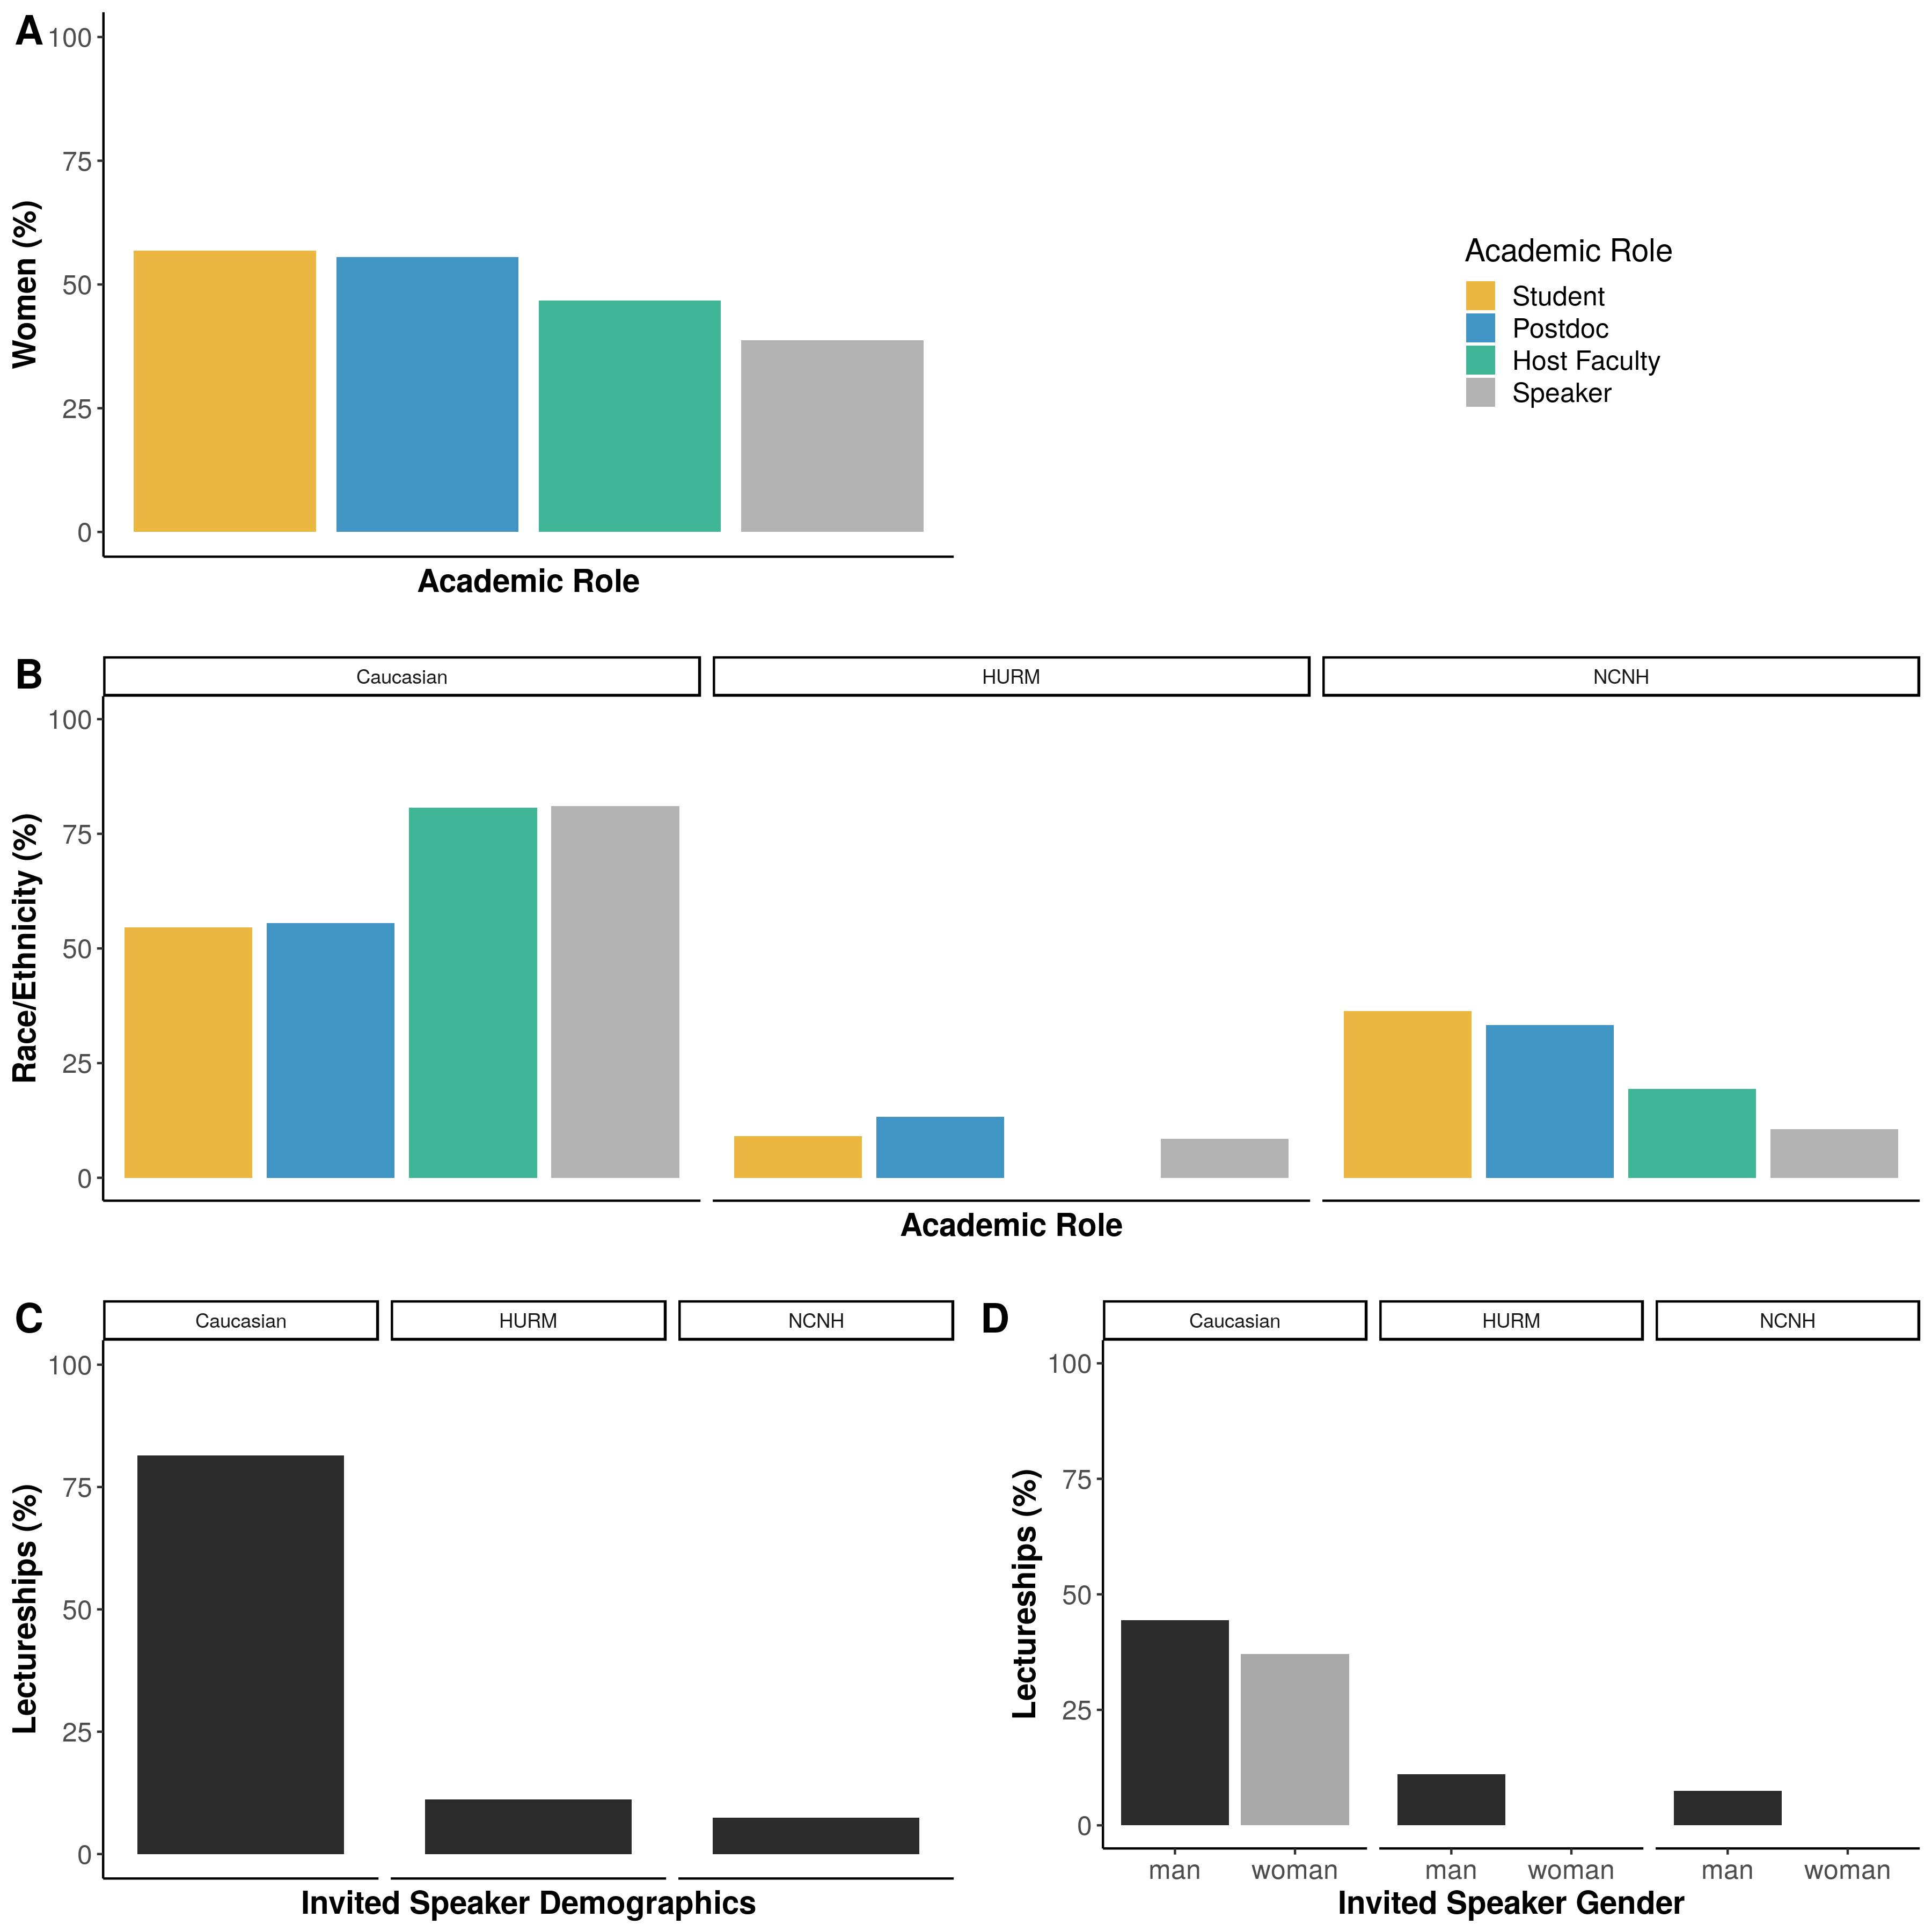
\includegraphics{Figure_1.jpg}
\caption{\textbf{The demographics of invited speakers, hosting faculty,
and trainees.} A) The proportion of women in each academic role. B) The
proportion of each academic role represented by individuals that are
Caucasian (left), Historically Underrepresented Minorities (HURM,
center) or Non-Caucasian/Non-HURM (NCNH, right). C-D)The percent of
lectureships awarded to individuals that are C) Caucasian, HURM, or NCNH
and D) Caucasian, HURM, or NCNH by gender.}
\end{figure}

\newpage

\subsection*{References}\label{references}
\addcontentsline{toc}{subsection}{References}

\hypertarget{refs}{}
\hypertarget{ref-Martinez2018}{}
1. \textbf{Martinez LR}, \textbf{Boucaud DW}, \textbf{Casadevall A},
\textbf{August A}. 2018. Factors contributing to the success of
NIH-designated underrepresented minorities in academic and nonacademic
research positions. CBELife Sciences Education \textbf{17}:ar32.
doi:\href{https://doi.org/10.1187/cbe.16-09-0287}{10.1187/cbe.16-09-0287}.

\hypertarget{ref-AllenRamdial2014}{}
2. \textbf{Allen-Ramdial S-AA}, \textbf{Campbell AG}. 2014. Reimagining
the pipeline: Advancing STEM diversity, persistence, and success.
BioScience \textbf{64}:612--618.
doi:\href{https://doi.org/10.1093/biosci/biu076}{10.1093/biosci/biu076}.

\hypertarget{ref-Fang2000}{}
3. \textbf{Fang D}. 2000. Racial and ethnic disparities in faculty
promotion in academic medicine. JAMA \textbf{284}:1085.
doi:\href{https://doi.org/10.1001/jama.284.9.1085}{10.1001/jama.284.9.1085}.

\hypertarget{ref-Gibbs2014}{}
4. \textbf{Gibbs KD}, \textbf{McGready J}, \textbf{Bennett JC},
\textbf{Griffin K}. 2014. Biomedical science ph.D. career interest
patterns by race/ethnicity and gender. PLoS ONE \textbf{9}:e114736.
doi:\href{https://doi.org/10.1371/journal.pone.0114736}{10.1371/journal.pone.0114736}.

\hypertarget{ref-Meyers2018}{}
5. \textbf{Meyers LC}, \textbf{Brown AM}, \textbf{Moneta-Koehler L},
\textbf{Chalkley R}. 2018. Survey of checkpoints along the pathway to
diverse biomedical research faculty. PLOS ONE \textbf{13}:e0190606.
doi:\href{https://doi.org/10.1371/journal.pone.0190606}{10.1371/journal.pone.0190606}.

\hypertarget{ref-nsf_2014}{}
6. \textbf{National Center for Science and Engineering Statistics}.
2014. Women, minorities, and persons with disabilities in science and
engineering. National Science Foundation, Alexandria, VA.

\hypertarget{ref-Jena2015}{}
7. \textbf{Jena AB}, \textbf{Khullar D}, \textbf{Ho O}, \textbf{Olenski
AR}, \textbf{Blumenthal DM}. 2015. Sex differences in academic rank in
US medical schools in 2014. JAMA \textbf{314}:1149.
doi:\href{https://doi.org/10.1001/jama.2015.10680}{10.1001/jama.2015.10680}.

\hypertarget{ref-Rotbart2012}{}
8. \textbf{Rotbart HA}, \textbf{McMillen D}, \textbf{Taussig H},
\textbf{Daniels SR}. 2012. Assessing gender equity in a large academic
department of pediatrics. Academic Medicine \textbf{87}:98--104.
doi:\href{https://doi.org/10.1097/acm.0b013e31823be028}{10.1097/acm.0b013e31823be028}.

\hypertarget{ref-Coe2019}{}
9. \textbf{Coe IR}, \textbf{Wiley R}, \textbf{Bekker L-G}. 2019.
Organisational best practices towards gender equality in science and
medicine. The Lancet \textbf{393}:587--593.
doi:\href{https://doi.org/10.1016/s0140-6736(18)33188-x}{10.1016/s0140-6736(18)33188-x}.

\hypertarget{ref-Firth1982}{}
10. \textbf{Firth M}. 1982. Sex discrimination in job opportunities for
women. Sex Roles \textbf{8}:891--901.
doi:\href{https://doi.org/10.1007/bf00287858}{10.1007/bf00287858}.

\hypertarget{ref-Correll2007}{}
11. \textbf{Correll SJ}, \textbf{Benard S}, \textbf{Paik I}. 2007.
Getting a job: Is there a motherhood penalty? American Journal of
Sociology \textbf{112}:1297--1339.
doi:\href{https://doi.org/10.1086/511799}{10.1086/511799}.

\hypertarget{ref-Fuegen2004}{}
12. \textbf{Fuegen K}, \textbf{Biernat M}, \textbf{Haines E},
\textbf{Deaux K}. 2004. Mothers and fathers in the workplace: How gender
and parental status influence judgments of job-related competence.
Journal of Social Issues \textbf{60}:737--754.
doi:\href{https://doi.org/10.1111/j.0022-4537.2004.00383.x}{10.1111/j.0022-4537.2004.00383.x}.

\hypertarget{ref-BlairLoy2017}{}
13. \textbf{Blair-Loy M}, \textbf{Rogers L}, \textbf{Glaser D},
\textbf{Wong Y}, \textbf{Abraham D}, \textbf{Cosman P}. 2017. Gender in
engineering departments: Are there gender differences in interruptions
of academic job talks? Social Sciences \textbf{6}:29.
doi:\href{https://doi.org/10.3390/socsci6010029}{10.3390/socsci6010029}.

\hypertarget{ref-noauthor_seeking_2013}{}
14. \textbf{National Research Council \textnormal{Policy and Global
Affairs}}, \textbf{Committee on Women in Science, Engineering, and
Medicine}, \textbf{Committee on Advancing Institutional Transformation
for Minority Women in Academia}, \textbf{Rapporteur KM}. 2013. Seeking
Solutions: Maximizing American Talent by Advancing Women of Color in
Academia: Summary of a Conference. National Academies Press, Washington,
D.C.

\hypertarget{ref-McGee2018}{}
15. \textbf{McGee E}. 2018. Black genius, asian fail: The detriment of
stereotype lift and stereotype threat in high-achieving asian and black
STEM students. AERA Open \textbf{4}:233285841881665.
doi:\href{https://doi.org/10.1177/2332858418816658}{10.1177/2332858418816658}.

\hypertarget{ref-wse_2016}{}
16. \textbf{Joan C. Williams RR \textnormal{Su Li}}, \textbf{Finn P}.
2016. Climate control: Gender and racial bias in engineering. University
of California Hastings College of the Law, San Francisco, CA.

\hypertarget{ref-pololi_race_2010}{}
17. \textbf{Pololi L}, \textbf{Cooper LA}, \textbf{Carr P}. 2010. Race,
Disadvantage and Faculty Experiences in Academic Medicine. Journal of
General Internal Medicine \textbf{25}:1363--1369.
doi:\href{https://doi.org/10.1007/s11606-010-1478-7}{10.1007/s11606-010-1478-7}.

\hypertarget{ref-hassouneh_experiences_2014}{}
18. \textbf{Hassouneh D}, \textbf{Lutz KF}, \textbf{Beckett AK},
\textbf{Junkins EP}, \textbf{Horton LL}. 2014. The experiences of
underrepresented minority faculty in schools of medicine. Medical
Education Online \textbf{19}:24768.
doi:\href{https://doi.org/10.3402/meo.v19.24768}{10.3402/meo.v19.24768}.

\hypertarget{ref-Herrmann2016}{}
19. \textbf{Herrmann SD}, \textbf{Adelman RM}, \textbf{Bodford JE},
\textbf{Graudejus O}, \textbf{Okun MA}, \textbf{Kwan VSY}. 2016. The
effects of a female role model on academic performance and persistence
of women in STEM courses. Basic and Applied Social Psychology
\textbf{38}:258--268.
doi:\href{https://doi.org/10.1080/01973533.2016.1209757}{10.1080/01973533.2016.1209757}.

\hypertarget{ref-Drury2011}{}
20. \textbf{Drury BJ}, \textbf{Siy JO}, \textbf{Cheryan S}. 2011. When
do female role models benefit women? The importance of differentiating
recruitment from retention in STEM. Psychological Inquiry
\textbf{22}:265--269.
doi:\href{https://doi.org/10.1080/1047840x.2011.620935}{10.1080/1047840x.2011.620935}.

\hypertarget{ref-Lambert2020}{}
21. \textbf{Lambert WM}, \textbf{Wells MT}, \textbf{Cipriano MF},
\textbf{Sneva JN}, \textbf{Morris JA}, \textbf{Golightly LM}. 2020.
Career choices of underrepresented and female postdocs in the biomedical
sciences. eLife \textbf{9}.
doi:\href{https://doi.org/10.7554/elife.48774}{10.7554/elife.48774}.

\hypertarget{ref-Hardeman2018}{}
22. \textbf{Hardeman RR}, \textbf{Murphy KA}, \textbf{Karbeah J},
\textbf{Kozhimannil KB}. 2018. Naming institutionalized racism in the
public health literature: A systematic literature review. Public Health
Reports \textbf{133}:240--249.
doi:\href{https://doi.org/10.1177/0033354918760574}{10.1177/0033354918760574}.

\hypertarget{ref-harvey_diversity_2011}{}
23. \textbf{Harvey WB}. 2011. Higher education and diversity: Ethical
and practical responsiblity in the academy.

\hypertarget{ref-Stack2019}{}
24. \textbf{Stack M}. 2019. Academic stars and university rankings in
higher education: Impacts on policy and practice. Policy Reviews in
Higher Education \textbf{4}:4--24.
doi:\href{https://doi.org/10.1080/23322969.2019.1667859}{10.1080/23322969.2019.1667859}.

\hypertarget{ref-Iverson2007}{}
25. \textbf{Iverson SV}. 2007. Camouflaging power and privilege: A
critical race analysis of university diversity policies. Educational
Administration Quarterly \textbf{43}:586--611.
doi:\href{https://doi.org/10.1177/0013161x07307794}{10.1177/0013161x07307794}.

\hypertarget{ref-Tate2016}{}
26. \textbf{Tate SA}, \textbf{Bagguley P}. 2016. Building the
anti-racist university: Next steps. Race Ethnicity and Education
\textbf{20}:289--299.
doi:\href{https://doi.org/10.1080/13613324.2016.1260227}{10.1080/13613324.2016.1260227}.

\hypertarget{ref-Gibbs2016}{}
27. \textbf{Gibbs KD}, \textbf{Basson J}, \textbf{Xierali IM},
\textbf{Broniatowski DA}. 2016. Decoupling of the minority PhD talent
pool and assistant professor hiring in medical school basic science
departments in the US. eLife \textbf{5}.
doi:\href{https://doi.org/10.7554/elife.21393}{10.7554/elife.21393}.

\hypertarget{ref-nittrouer_gender_2018}{}
28. \textbf{Nittrouer CL}, \textbf{Hebl MR}, \textbf{Ashburn-Nardo L},
\textbf{Trump-Steele RCE}, \textbf{Lane DM}, \textbf{Valian V}. 2018.
Gender disparities in colloquium speakers at top universities.
Proceedings of the National Academy of Sciences \textbf{115}:104--108.
doi:\href{https://doi.org/10.1073/pnas.1708414115}{10.1073/pnas.1708414115}.

\hypertarget{ref-kalejta_gender_2017}{}
29. \textbf{Kalejta RF}, \textbf{Palmenberg AC}. 2017. Gender Parity
Trends for Invited Speakers at Four Prominent Virology Conference
Series. Journal of Virology \textbf{91}.
doi:\href{https://doi.org/10.1128/JVI.00739-17}{10.1128/JVI.00739-17}.

\hypertarget{ref-casadevall_presence_2014}{}
30. \textbf{Casadevall A}, \textbf{Handelsman J}. 2014. The Presence of
Female Conveners Correlates with a Higher Proportion of Female Speakers
at Scientific Symposia. mBio \textbf{5}.
doi:\href{https://doi.org/10.1128/mBio.00846-13}{10.1128/mBio.00846-13}.

\hypertarget{ref-klein_speaking_2017}{}
31. \textbf{Klein RS}, \textbf{Voskuhl R}, \textbf{Segal BM},
\textbf{Dittel BN}, \textbf{Lane TE}, \textbf{Bethea JR}, \textbf{Carson
MJ}, \textbf{Colton C}, \textbf{Rosi S}, \textbf{Anderson A},
\textbf{Piccio L}, \textbf{Goverman JM}, \textbf{Benveniste EN},
\textbf{Brown MA}, \textbf{Tiwari-Woodruff SK}, \textbf{Harris TH},
\textbf{Cross AH}. 2017. Speaking out about gender imbalance in invited
speakers improves diversity. Nature Immunology \textbf{18}:475--478.
doi:\href{https://doi.org/10.1038/ni.3707}{10.1038/ni.3707}.

\hypertarget{ref-Broderick2019}{}
32. \textbf{Broderick NA}, \textbf{Casadevall A}. 2019. Gender
inequalities among authors who contributed equally. eLife \textbf{8}.
doi:\href{https://doi.org/10.7554/elife.36399}{10.7554/elife.36399}.

\hypertarget{ref-Kimery2011}{}
33. \textbf{Kimery KM}, \textbf{Mellon MJ}, \textbf{Rinehart SM}. 2011.
Publishing in the accounting journals: Is there a gender bias? Journal
of Business \& Economics Research (JBER) \textbf{2}.
doi:\href{https://doi.org/10.19030/jber.v2i4.2872}{10.19030/jber.v2i4.2872}.

\hypertarget{ref-Helmer2017}{}
34. \textbf{Helmer M}, \textbf{Schottdorf M}, \textbf{Neef A},
\textbf{Battaglia D}. 2017. Gender bias in scholarly peer review. eLife
\textbf{6}.
doi:\href{https://doi.org/10.7554/elife.21718}{10.7554/elife.21718}.

\hypertarget{ref-Fox2019}{}
35. \textbf{Fox CW}, \textbf{Paine CET}. 2019. Gender differences in
peer review outcomes and manuscript impact at six journals of ecology
and evolution. Ecology and Evolution \textbf{9}:3599--3619.
doi:\href{https://doi.org/10.1002/ece3.4993}{10.1002/ece3.4993}.

\hypertarget{ref-Gilbert1994}{}
36. \textbf{Gilbert JR}. 1994. Is there gender bias in JAMAs peer review
process? JAMA: The Journal of the American Medical Association
\textbf{272}:139.
doi:\href{https://doi.org/10.1001/jama.1994.03520020065018}{10.1001/jama.1994.03520020065018}.

\hypertarget{ref-Okonofua2013}{}
37. \textbf{Okonofua BA}. 2013. I am blacker than you. SAGE Open
\textbf{3}:215824401349916.
doi:\href{https://doi.org/10.1177/2158244013499162}{10.1177/2158244013499162}.

\hypertarget{ref-R_software_2017}{}
38. \textbf{R Core Team}. 2017. R: A language and environment for
statistical computing. R Foundation for Statistical Computing, Vienna,
Austria.

\hypertarget{ref-wickham_tidyverse_2017}{}
39. \textbf{Wickham H}. 2017. Tidyverse: Easily Install and Load the
'Tidyverse'.

\hypertarget{ref-cowplot}{}
40. \textbf{Wilke CO}. 2019. Cowplot: Streamlined plot theme and plot
annotations for 'ggplot2'.

\hypertarget{ref-markdown}{}
41. \textbf{Allaire J}, \textbf{Horner J}, \textbf{Xie Y}, \textbf{Marti
V}, \textbf{Porte N}. 2018. Markdown: 'Markdown' rendering for r.

\hypertarget{ref-rmd_book}{}
42. \textbf{Xie Y}, \textbf{Allaire J}, \textbf{Grolemund G}. 2018. R
markdown: The definitive guide. Chapman; Hall/CRC, Boca Raton, Florida.

\hypertarget{ref-rmd_rstudio}{}
43. \textbf{Allaire J}, \textbf{Xie Y}, \textbf{McPherson J},
\textbf{Luraschi J}, \textbf{Ushey K}, \textbf{Atkins A},
\textbf{Wickham H}, \textbf{Cheng J}, \textbf{Chang W}, \textbf{Iannone
R}. 2018. Rmarkdown: Dynamic documents for r.

\hypertarget{ref-knitr_2014}{}
44. \textbf{Xie Y}. 2014. Knitr: A comprehensive tool for reproducible
research in R. \emph{In} Stodden, V, Leisch, F, Peng, RD (eds.),
Implementing reproducible computational research. Chapman; Hall/CRC.

\hypertarget{ref-knitr_2018}{}
45. \textbf{Xie Y}. 2018. Knitr: A general-purpose package for dynamic
report generation in r.

\hypertarget{ref-lubridate}{}
46. \textbf{Grolemund G}, \textbf{Wickham H}. 2011. Dates and times made
easy with lubridate. Journal of Statistical Software \textbf{40}:1--25.

\hypertarget{ref-readxl}{}
47. \textbf{Wickham H}, \textbf{Bryan J}. 2018. Readxl: Read excel
files.

\hypertarget{ref-pdftools}{}
48. \textbf{Ooms J}. 2019. Pdftools: Text extraction, rendering and
converting of pdf documents.

\hypertarget{ref-wickham_scales_2018}{}
49. \textbf{Wickham H}. 2018. Scales: Scale Functions for Visualization.

\hypertarget{ref-neuwirth_rcolorbrewer_2014}{}
50. \textbf{Neuwirth E}. 2014. RColorBrewer: ColorBrewer Palettes.

\hypertarget{ref-nsf_survey_2017}{}
51. \textbf{National Center for Science and Engineering Statistics}.
2017. Survey of Doctorate Recipients, Survey Year 2017. National Science
Foundation, Alexandria, VA.

\hypertarget{ref-Crenshaw1989}{}
52. \textbf{Crenshaw K}. 1989. Demarginalizing the Intersection of Race
and Sex: A black feminist critique of antidiscrimination doctrine,
feminist theory and antiracist politics. University of Chicago Legal
Forum \textbf{1989}.
doi:\href{https://doi.org/10.1007/s11162-008-9097-4}{10.1007/s11162-008-9097-4}.

\hypertarget{ref-nsf_2019}{}
53. \textbf{National Center for Science and Engineering Statistics
Directorate for Social, Behavioral, and Economic Sciences}. 2019. Women,
minorities, and persons with disabilities in science and engineering.
National Science Foundation, Alexandria, VA.

\hypertarget{ref-allagnat_gender_2017}{}
54. \textbf{Allagnat L}, \textbf{Berghmans S}, \textbf{Falk-Krzesinski
HJ}, \textbf{Hanafi S}, \textbf{Herbert R}, \textbf{Huggett S},
\textbf{Tobin S}. 2017. Gender in the global research landscape.

\hypertarget{ref-Armstrong2015}{}
55. \textbf{Armstrong MA}, \textbf{Jovanovic J}. 2015. STARTING AT THE
CROSSROADS: INTERSECTIONAL APPROACHES TO INSTITUTIONALLY SUPPORTING
UNDERREPRESENTED MINORITY WOMEN STEM FACULTY. Journal of Women and
Minorities in Science and Engineering \textbf{21}:141--157.
doi:\href{https://doi.org/10.1615/jwomenminorscieneng.2015011275}{10.1615/jwomenminorscieneng.2015011275}.

\hypertarget{ref-xu_gender_2008}{}
56. \textbf{Xu YJ}. 2008. Gender Disparity in STEM Disciplines: A Study
of Faculty Attrition and Turnover Intentions. Research in Higher
Education \textbf{49}:607--624.
doi:\href{https://doi.org/10.1007/s11162-008-9097-4}{10.1007/s11162-008-9097-4}.

\hypertarget{ref-whittaker_retention_2015}{}
57. \textbf{Whittaker JA}, \textbf{Montgomery BL}, \textbf{Martinez
Acosta VG}. 2015. Retention of Underrepresented Minority Faculty:
Strategic Initiatives for Institutional Value Proposition Based on
Perspectives from a Range of Academic Institutions. Journal of
undergraduate neuroscience education: JUNE: a publication of FUN,
Faculty for Undergraduate Neuroscience \textbf{13}:A136--145.

\hypertarget{ref-johnson_msphere_2019}{}
58. \textbf{Johnson MDL}. 2019. mSphere of Influence: Hiring of
Underrepresented Minority Assistant Professors in Medical School Basic
Science Departments Has a Long Way To Go. mSphere \textbf{4}.
doi:\href{https://doi.org/10.1128/mSphere.00599-19}{10.1128/mSphere.00599-19}.

\hypertarget{ref-Loftus1971}{}
59. \textbf{Loftus GR}. 1971. Comparison of recognition and recall in a
continuous memory task. Journal of Experimental Psychology
\textbf{91}:220--226.
doi:\href{https://doi.org/10.1037/h0031841}{10.1037/h0031841}.

\hypertarget{ref-Johnson2014}{}
60. \textbf{Johnson J}. 2014. Recognition is easy\(\mathsemicolon\)
recall is hard, pp. 121--129. \emph{In} Designing with the mind in mind.
Elsevier.

\hypertarget{ref-Baucom_2019}{}
61. \textbf{Baucom R}, \textbf{Duffy M}. 2019. DiversifyEEB.
\url{https://diversifyeeb.com}.

\hypertarget{ref-Duffy_2019}{}
62. \textbf{Duffy M}, \textbf{McNeil AJ}. 2019. DiversifyChemistry.
\url{https://diversifychemistry.com}.

\hypertarget{ref-Hagan2019_micro}{}
63. \textbf{Hagan AK}, \textbf{Pollet RM}. 2019. DiversifyMicrobiology.
GitHub repository.
\url{https://github.com/diversifymicrobiology.github.io}; GitHub.

\hypertarget{ref-Hagan2019_immuno}{}
64. \textbf{Hagan AK}, \textbf{Pollet RM}. 2019. DiversifyImmunology.
GitHub repository.
\url{https://github.com/diversifyimmunology.github.io}; GitHub.


\end{document}
